\documentclass[12pt]{article}
\usepackage[utf8]{inputenc}
\usepackage{float}
\usepackage{amsmath}
\usepackage{graphicx}

\usepackage[hmargin=3cm,vmargin=6.0cm]{geometry}
%\topmargin=0cm
\topmargin=-2cm
\addtolength{\textheight}{6.5cm}
\addtolength{\textwidth}{2.0cm}
%\setlength{\leftmargin}{-5cm}
\setlength{\oddsidemargin}{0.0cm}
\setlength{\evensidemargin}{0.0cm}

%misc libraries goes here



\begin{document}

\section*{Student Information } 
%Write your full name and id number between the colon and newline
%Put one empty space character after colon and before newline
Full Name : Emre Geçit \\
Id Number : 2521581\\

% Write your answers below the section tags
\section*{Answer 1}
$\sum_{n=1}^{\infty} a_nx^{n} = \sum_{n=1}^{\infty} a_{n-1}x^{n-1} + \sum_{n=1}^{\infty}2^nx^{n}\\\\
\sum_{n=1}^{\infty} a_nx^{n} = \sum_{n=1}^{\infty} a_{n-1}x^{n-1} + \sum_{n=1}^{\infty}u^{n}$ (substitute 2x with u)$\\\\
A(x)-1=A(x)*x+\sum_{n=1}^{\infty}u^{n}\\\\
A(x)-1=A(x)*x+\dfrac{1}{1-u}\\\\
A(x)-1=A(x)*x+\dfrac{1}{1-2x}\\\\
(x-1)*A(x)=\dfrac{1}{1-2x}\\\\
A(x)=\dfrac{1}{(1-2x)*(x-1)}\\\\
A(x)=\dfrac{2}{1-2x}+\dfrac{-1}{1-x}$ (partial fractions)
$\\\\A(x)=-1*(1,1,1,...,1,...)+2*(1,2,4,...,2^n,...)\\\\
a_n=-1+2*2^n\\\\
a_n=2^{n+1}-1\\\\$

\section*{Answer 2}
a) Hasse diagram of R:\\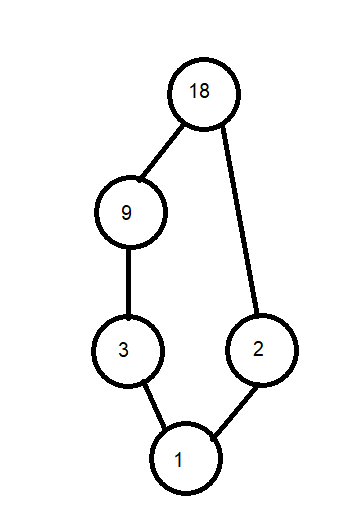
\includegraphics{HASS.png}\\
b) Matrix representation of R:$\begin{pmatrix}
1 & 1 & 1 & 1 & 1\\
0 & 1 & 0 & 0 & 1\\
0 & 0 & 1 & 1 & 1\\
0 & 0 & 0 & 1 & 1\\
0 & 0 & 0 & 0 & 1
\end{pmatrix}\\\\\\$
c) None of the pairs have more than one Greatest Lower Bound or Lowest Upper Bound, therefore (A, R) is a lattice.\\\\
d) $R_s=R \cup R^{-1}\\\\
R = \begin{pmatrix}
1 & 1 & 1 & 1 & 1\\
0 & 1 & 0 & 0 & 1\\
0 & 0 & 1 & 1 & 1\\
0 & 0 & 0 & 1 & 1\\
0 & 0 & 0 & 0 & 1
\end{pmatrix}\\\\\\
R^{-1}=\begin{pmatrix}
1 & 0 & 0 & 0 & 0\\
1 & 1 & 0 & 0 & 0\\
1 & 0 & 1 & 0 & 0\\
1 & 0 & 1 & 1 & 0\\
1 & 1 & 1 & 1 & 1
\end{pmatrix}\\\\\\
R_s=R_s=R \cup R^{-1}=\begin{pmatrix}
1 & 1 & 1 & 1 & 1\\
1 & 1 & 0 & 0 & 1\\
1 & 0 & 1 & 1 & 1\\
1 & 0 & 1 & 1 & 1\\
1 & 1 & 1 & 1 & 1
\end{pmatrix}\\\\\\$
e) 2 and 9 are not comparable since $2|9$ and $9|2$ are both false, 3 and 18 are comparable since $3|18$ is true.
\section*{Answer 3}
a) For the diagonal there can be $2^n$ possibilities. For the cells that are not in the diagonal, for each symmetric pair of cells, there can be 3 possible states ((0,0),(0,1),(1,0)). There are $(n^2-n)/2$ symmetric cell pairs. Therefore, there are $2^n * 3^{(n^2-n)/2}$ possible binary anti-symmetric relations for a set with n elements.\\\\b) For a reflexive relation, the diagonal should be filled with ones, so for the diagonal there is one possibility. For the cells that are not in the diagonal, for each symmetric pair of cells, there can be 3 possible states ((0,0),(0,1),(1,0)). There are $(n^2-n)/2$ symmetric cell pairs. Therefore, there are $3^{(n^2-n)/2}$ possible binary, reflexive and anti-symmetric relations for a set with n elements.

\end{document}